\documentclass[usenatbib,fleqn]{mnras}

\pdfoutput=1

\usepackage{amsmath}
\usepackage{amssymb}
\usepackage{blindtext}
\usepackage{bm}
\usepackage{color}
\usepackage{graphicx}
\usepackage{hyperref}
\usepackage[all]{hypcap}
% \usepackage{lineno}
\usepackage{longtable}
\usepackage{multicol}
\usepackage{multirow}
\usepackage{natbib}
% \usepackage{flushend}
\usepackage{txfonts}
\usepackage{wasysym}
\usepackage[capitalize,nameinlink]{cleveref}

% cleveref tweak to remove parentheses from equations
\creflabelformat{equation}{#2#1#3}
\crefrangelabelformat{equation}{#3#1#4 to #5#2#6}

% For links of references
\hypersetup{colorlinks,
  linkcolor=red,
  filecolor=red,
  urlcolor=magenta,
  citecolor=blue}

\usepackage{array}
\newcolumntype{L}[1]{>{\raggedright\let\newline\\\arraybackslash\hspace{0pt}}m{#1}}
\newcolumntype{C}[1]{>{\centering\let\newline\\\arraybackslash\hspace{0pt}}m{#1}}
\newcolumntype{R}[1]{>{\raggedleft\let\newline\\\arraybackslash\hspace{0pt}}m{#1}}

\newcommand{\comment}[1]{\textbf{\color{magenta} #1}}

\newcommand{\Msun}{\mathrm{M}_\odot}
\newcommand{\hMsun}{h^{-1}\,\Msun}
\newcommand{\hMpc}{h^{-1}\,\mathrm{Mpc}}
\newcommand{\subfind}{\textsc{subfind}}


\title[Mass content of satellites in EAGLE]{The effect of massive clusters on the mass of galaxies in their vicinity}

\author[C.\ Sif\'on]{Crist\'obal Sif\'on
\\
Department of Astrophysical Sciences, Peyton Hall, Princeton University, Princeton, NJ 08544, USA
}

% These dates will be filled out by the publisher
% \date{Accepted XXX. Received YYY; in original form ZZZ}

% Enter the current year, for the copyright statements etc.
\pubyear{2018}

\begin{document}
\label{firstpage}
\pagerange{\pageref{firstpage}--\pageref{lastpage}}

% \linenumbers

\maketitle

\begin{abstract}
  We use the EAGLE hydrodynamical simulation to explore the infall of galaxies into massive ($M_{200m}>10^{13}\,\Msun$) galaxy groups and clusters, paying particular attention to their changing density profiles.
  
  We explore changes in satellite stellar mass/halo mass as a function of (the observationally accessible) distance from host/nearest cluster, as well as the more physical change as a function of time for the same satellites.
  
  We identify the progenitors of $z=0.18$ satellites as \textbf{some population of centrals at some earlier time}, and find \textbf{the following problems arise when interpreting differences between present-day satellites with present-day centrals}

\end{abstract}



\section{Wish/thought list}

(Given in the order they came to my head)

\begin{enumerate}
  \item The distribution of distances to closest group makes a lot more sense than that within the host group. This may have to do with some satellites being ``2nd-order'' subhaloes, i.e., being part of a larger \emph{sub}halo. Explore this by exemplifying with the most massive cluster.
  \item Explore what difference does it make where did the satellite come from, by binning as a function of cluster-centric distance but also, for galaxies not part of the cluster, by host mass (probably do not need groups less massive than $10^{12}\,h^{-1}\,\Msun$, as that's already the mass of the Milky Way)
  \item try to find a good definition for subhalo size using the density profiles. Perhaps differences between our measurements and EAGLE are caused by a model error?
  \item Plot stellar-to-total mass ratios as a function of cluster-centric distance.
\end{enumerate}

\subsection{Important papers}

\begin{enumerate}
  \item \cite{vdbosch17}
  \item \cite{moline17} -- compare $c(M)$ relation; what's the effect of baryons?
\end{enumerate}

\section{Introduction}

In this paper we refer generically to ``galaxy groups'' as all galaxy associations more massive than $M_{200m}=10^{11}\,\hMsun$, and to ``clusters'' as the subset of those groups which have $M_{200m}>10^{13}\,\Msun$. (This is a more relaxed definition of ``cluster'' than usual.) Throughout, we refer to masses $M_{\Delta m}$ ($M_{\Delta c}$) as the mass containing $\Delta$ times the mean (critical) density of the Universe at the group redshift. Where appropriate, we adopt the cosmology used in the EAGLE simulations,  with \textbf{parameters...}


\section{Simulated galaxy sample}

Our study is based on the Evolution and Assembly of Galaxies and their Environment (EAGLE) simulations \citep{schaye15,crain15}. EAGLE is a suite of cosmological hydrodynamical simulations with varying box sizes, resolutions, and baryonic feedback prescriptions. The fiducial simulation we use for our study is labelled RefL0100N1504 and has a box size of $(100\,\hMpc)^3$, with N particles and X,Y,Z particle mass for dark matter, gas and stars, respectively.

Haloes were identified in EAGLE using a standard friends-of-friends algorithm with a linking length of X, and subhaloes were identified using \subfind\ \citep{springel01_cluster}. \cite{knebe11} found that \subfind\ tends to underpredict subhalo masses at all halo-centric distances. While uncertainties on the bias were not reported by \cite{knebe11}, the smooth behaviour of the bias as a function of halo-centric distance suggests that uncertainties are rather small, and we neglect them in our analysis. By interpolating figure 8 of \cite{knebe11}, we apply the following correction to all subhalo and galaxy masses reported in the EAGLE database:
\begin{equation}\label{eq:subfind_correction}
  \Delta m_\mathrm{sub}(x) = ...
\end{equation}
where $x=R/R_{200m}$ is the three-dimensional distance normalized by the halo size.\footnote{\cite{knebe11} reported their results in terms of $R_{200c}$ and $M_{200c}$. We convert from $R_{200c}$ to $R_{200m}$ using \textbf{a mass-concentration relation consistent with EAGLE -- look for one}.}

We adopt the location of the minimum of the gravitational potential as the position of all subhaloes, consistent with \cite{velliscig17}.

\Cref{f:massfunction} shows the mass functions of 

\begin{figure}
  \centerline{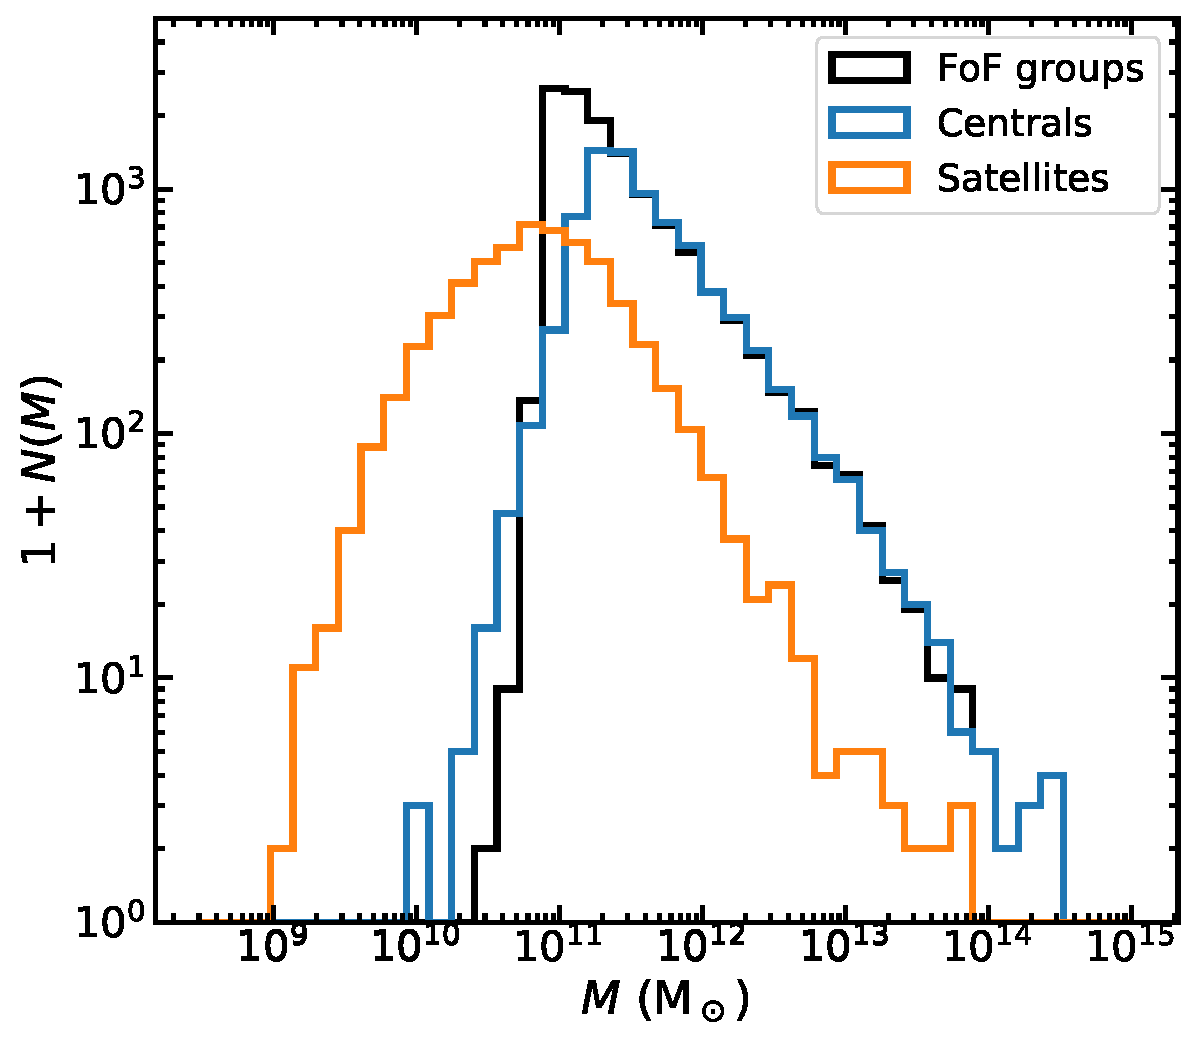
\includegraphics[width=\linewidth]{massfunction.pdf}}
\caption{Mass function of galaxy groups (left) and central and satellite galaxies (right) in the EAGLE RefL0100N1504 simulation. \textbf{Make single panel}}
\label{f:massfunction}
\end{figure}


\section{Data/Results/etc}

\begin{figure*}
  \centerline{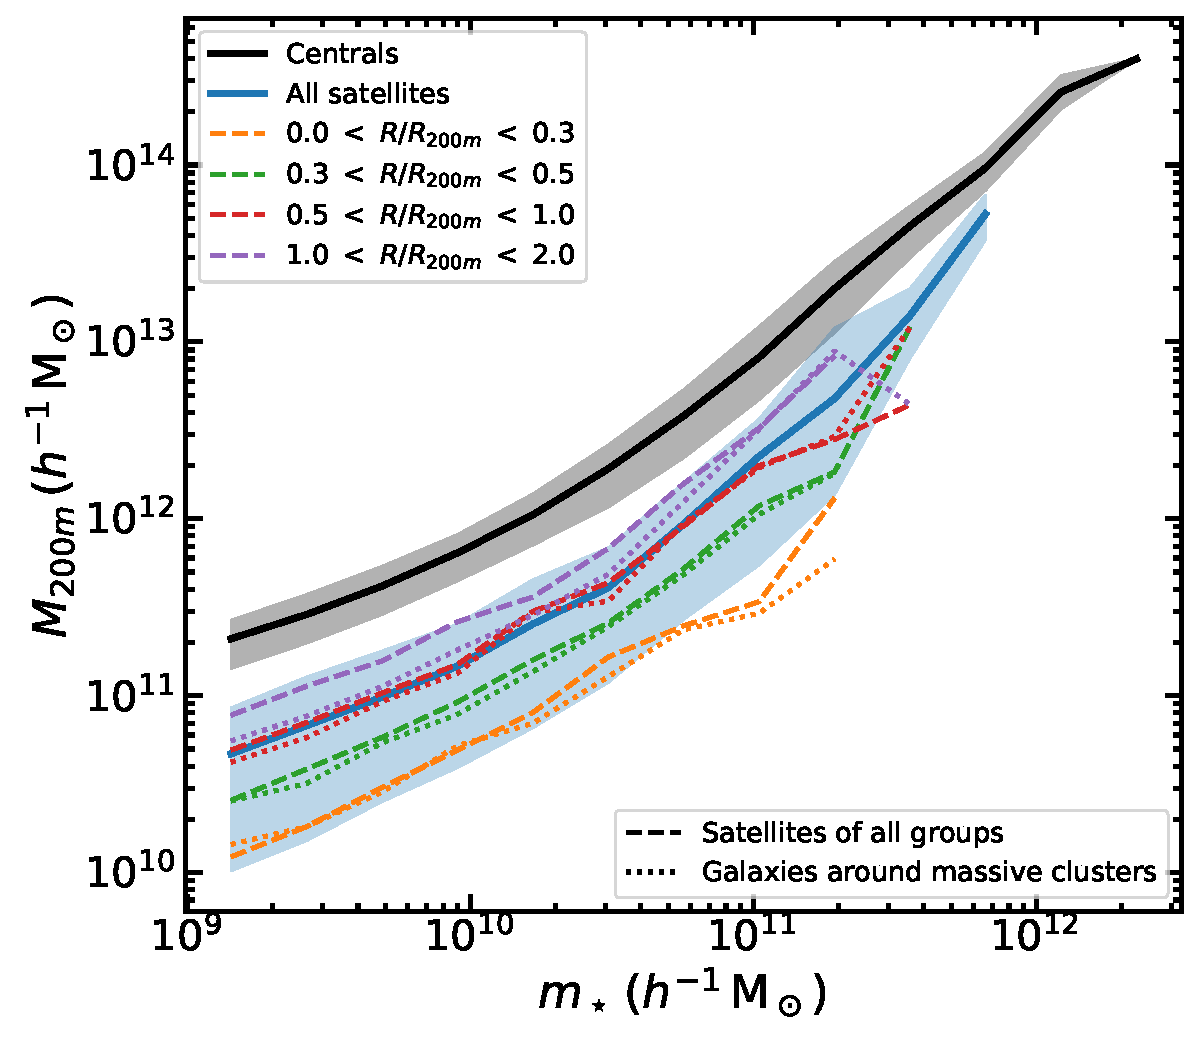
\includegraphics[width=\linewidth]{total_to_stellar_groups_and_clusters.pdf}}
\caption{The total-to-stellar mass relation of galaxies as a function of distance to their \emph{host} group (dashed lines), and as a function of their distance to the \emph{nearest} massive ($M_{200m}>10^{13}\,h^{-1}\,\Msun$) cluster (dotted lines), each normalized by the size of the group/cluster. The blue line shows the average total-to-stellar mass relation of all satellites belonging to all groups, and the black line shows the total-to-stellar mass relation of central galaxies. In the latter two, the respective shaded regions show the scatter in each.}
\label{f:relation}
\end{figure*}

\Cref{f:relation} shows that:
\begin{enumerate}
  \item the TSMR of subhaloes is approximately a factor 4 lower than that of centrals.
  \item the TSMR decreases in amplitude as we get closer to the cluster centre, but its shape does not change.
  \item If cluster size is accounted for, the TSMR of subhaloes does not depend on cluster mass (i.e., dashed and dotted lines of the same color overlap), except perhaps for low-mass galaxies outside $R_{200m}$. \emph{This suggests that massive clusters exert their influence out to larger radius compared to low-mass clusters}, especially for low-mass galaxies ($m_\mathrm{gal}\lesssim10^{-2}M_\mathrm{cl}$).
\end{enumerate}

Need to check how much of point (ii) may be caused by biases in subfind (compare to the curve of recovered versus true mass as a function of radius from Knebe+11).


\section{Application to satellite lensing measurements}


\bibliographystyle{mnras}
\bibliography{bibliography}






\end{document}


